\chapter{Konzeption der technischen Umsetzung}\label{chapter:tanforderungen}
Das Ziel des folgende Kapitel ist es zu erläutern wie auf Baisis der aufgestellten gesetzlichen und funktionalen Anforderungen ein der Zielsetzung dieser Arbeit entsprechenden Messenger Dienst erstellt werden kann. Das im folgenden Kapitel erstellte Konzept zur Umsetzung des Dienstes soll als Leitfaden für die reale Erstellung des Messengers dienen. 

\section{Framework als Basis des Konzepts}\label{chapter:kr}
Um die Umsetzbarkeit der aufgestellten Anforderungen an den Messenger Dienst in einem realistischen und ökonomischen Rahmen zu halten wird davon abgesehen ein komplett neues Messenger System von Grund auf Aufzubauen. Es ist wesentlich effizienter die Entwicklung des Messengers auf einem bestehenden Framework aufzubauen, welches sich den Anforderungen entsprechend Anpassen lässt. Das folgende Kapitel beschäftigt sich mit Frameworks, welche für die aufgabe infrage kommen, damit anschließend das Konzept zur Umsetzung des Messengers auf Basis des ausgewählten Frameworks entwickelt werden kann. 

\subsection{Auswahl des Frameworks}\label{chapter:am}
//Kapitel noch nicht wertig
Viele Open source Messenger mit denen sich die Anforderungen theoreitsich Umsetzen lassen

Grundlegende Kriterien: GDPR Compilance muss möglich sein, opensource und selbsthostbar

Matrix Framework: Robuste Basis, großer Fokus auf sicherheit, aktive Entwickelr Community, bietet Beispiel Interlation für Front und Backend, viele Anforderungen lassen sich gut mit Matrix umsetzen, dezentraliserit, wird für ähnliche Anwendugnsflälle bereits verwendet.

\subsection{Vorstellung des Matrix Frameworks}\label{chapter:vdmf}
Matrix ist ein offener Standard und ein Kommunikationsprotokoll für  Echtzeitkommunikation. Matrix bietet ein opensource Backend, welches über eine http API erreicht werden kann und die Kernfunktionen des Dienstes bereitstellt. Matrix bietet ebenfalls ein opensource Frontend, welches ein User Interface bereitstellt, über welches via der http API mit dem Backend kommuniziert werden kann. Somit stellt Matrix ein vollständiges, exemplarisches, opensource Backend und Frontend. Ein weiteres Alleinstellungsmerkmal von Matrix gegenüber anderer Standards ist zum einen, dass es mit einem besonderen Fokus auf Sicherheit entwickelt wurde und eine vollständig End zu End verschlüsselte Kommunikation  erlaubt, zum anderen, dass es dezentralisiert betrieben werden kann. Die Bedeutung der Dezentralisierung für die Umsetzung des Dienstes wird in späteren Kapiteln noch weiter erläutert.

Das Matrix-Projekt wurde von einer gemeinnützigen Stiftung mit Sitz in Großbritannien mit dem Ziel ins Leben gerufen, ein Framework für dezentrale Open-Source-Messaging-Dienste mit den Schwerpunkten Sicherheit, Datenschutz und Anpassungsfähigkeit zu entwickeln. Heute bietet Matrix eine robuste Codebasis zum Einrichten benutzerdefinierter Messaging-Dienste und bietet Element, eine ergänzende Slack-ähnliche Benutzeroberfläche.

Aufgrund seiner hohen Sicherheitsstandards und seines dezentralen Ansatzes wurde Matrix  von der französischen Regierung ausgewählt, um die Basis für eine sichere Instant Messenger-App zu schaffen und eine bessere Kommunikation in und zwischen verschiedenen Abteilungen der Regierung zu ermöglichen. Neben der französischen Regierung wählte auch die deutsche Bundeswehr Matrix als Basis für die Entwicklung eines internen Kommunikationsinstruments.

\subsubsection{Matrix Funktionsumfang für den Nutzer}\label{chapter:aemn}
Von Haus aus verfügt Matrix bereits über einen sehr robusten Funktionsumfang, welcher im Folgenden vorgestellt wird.
Der Aufbau des Dienstes ist mit dem von Slack vergleichbar. Das bedeutet Chats werden in Einzel/ Gruppenchats und Räume aufgeteilt. 

% Einfügen einer Grafik
\begin{figure}[htb]
    % Zentrierung
    \centering
    % Einfügen der Datei, mit angepasster Höhe
    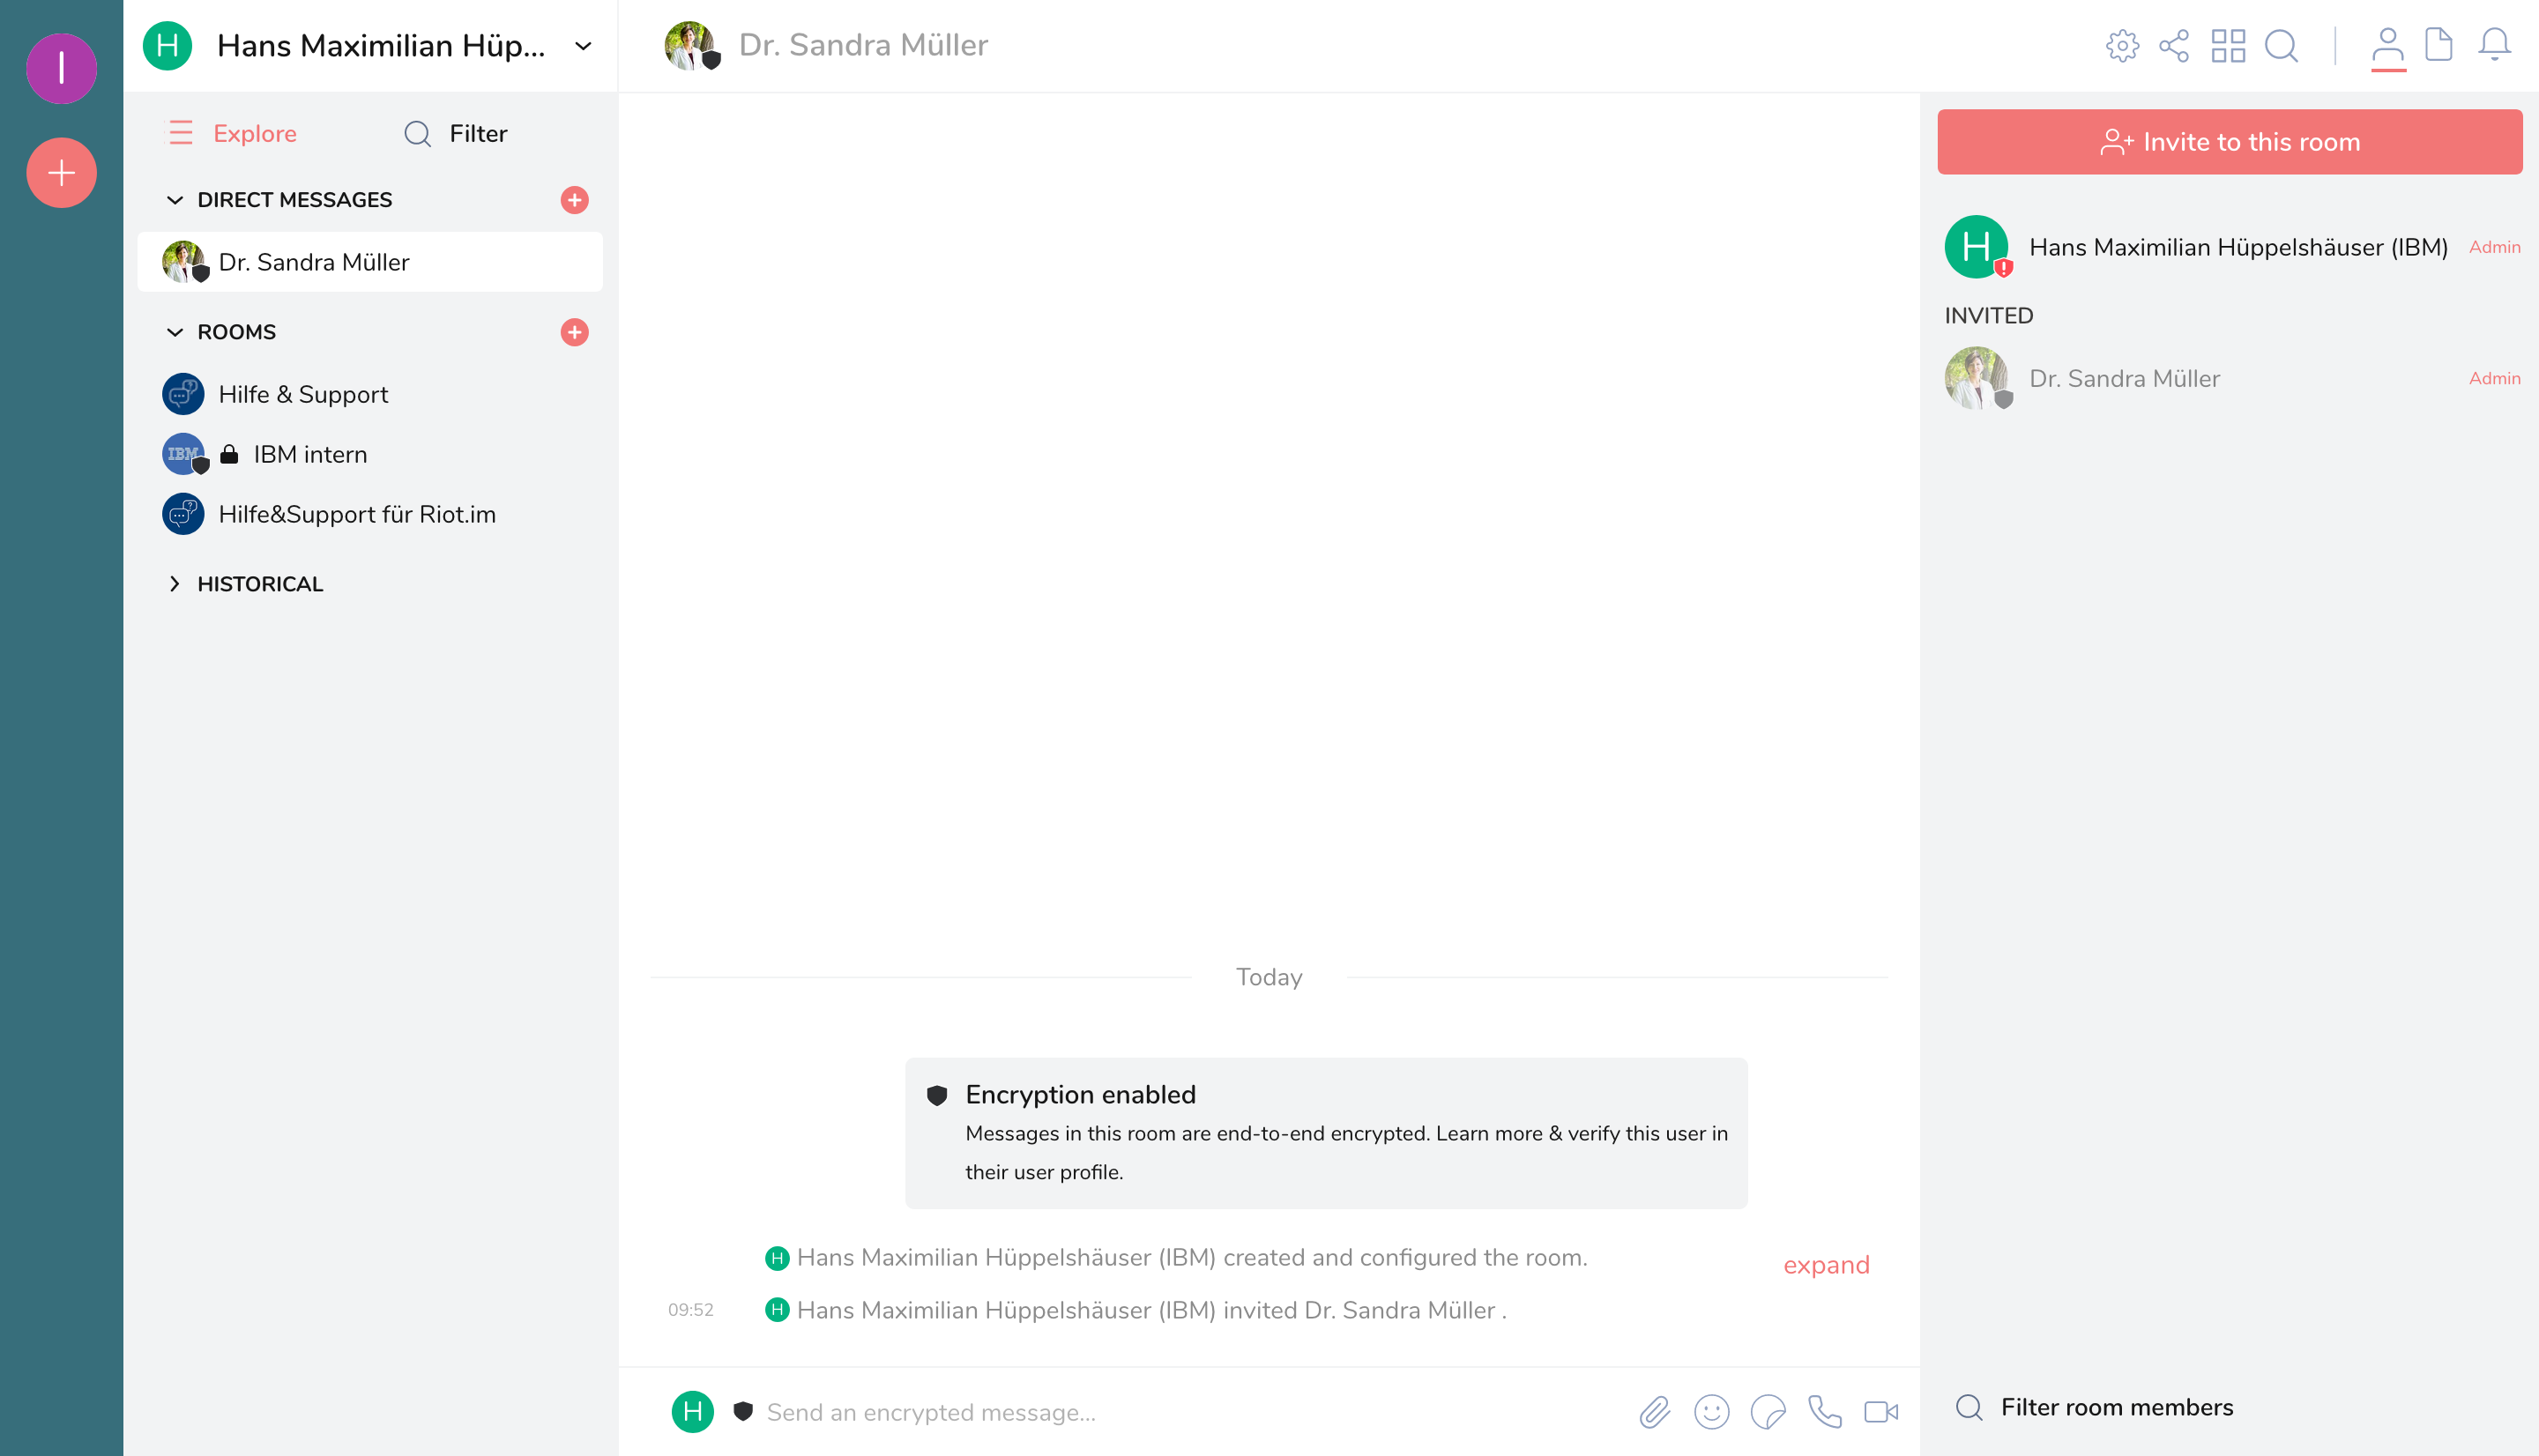
\includegraphics[height=8cm]{graphics/unknown-3.png}
    % Titel und Label der Grafik
    \caption[Matrix UI]{Matrix UI.\footnotemark}
    \label{abb:UI}
\end{figure}

Während Chats für den Austausch zwischen ausgewählten Personen ausgelegt sind, werden Räume Themen spezifisch angelegt. Räume lassen sich zudem auch öffentlich stellen, sodass sie von anderen Nutzern über eine Suche gefunden werden können. Desweiteren bietet Matrix die Möglichkeit Chats und Räume zu sogenannten Communitys zusammenzustellen, welche dabei helfen das Interface übersichtlich zu halten.
Neben der Suche nach Räumen ist Matrix auch in der Lage nach im System hinterlegten Nutzern zu suchen. Die Chats selber bieten die von anderen Messengern wie Slack bereits bekannte Funktionen, wie das Teilen von Dateien, das Senden von Emoticons, das Antworten auf spezifische Nachrichten in Form von Threads oder das Reagieren auf Nachrichten durch Emoticons. Chats und Räume lassen sich mit einer bereitgestellten Suchfunktion durchsuchen. Räume und Chats verfügen auch über weitreichende Optionen zur Administration, darunter ein robustes System zur Vergabe von Rechten an Nutzer, wie zum Beispiel das Recht darauf Nutzer zum Chat/ Raum hinzuzufügen oder zu entfernen, das Recht Nachrichten in der entsprechenden Gruppe zu verschicken oder Nachrichten zu löschen. Besonders relevant für die spätere Konzeption ist auch die Möglichkeit seitens Matrix Nachrichten nur für einen bestimmten Zeitraum zu speichern.
Neben den eigentlichen Chat Funktionen ist Matrix auch in der Lage Video und Audio Telefonate mit Einzelpersonen oder Gruppen führen.

Matrix erlaubt es dem Nutzer eine Reihe von Identifikatoren, wie E-Mail oder Telefonnummer im eigenen Nutzerprofil zu hinterlegen, ein Profilbild anzulegen, das Erscheinungsbild des Messengers zu personalisieren, oder das eigene Passwort zu ändern.

\subsubsection{Matrix Architektur}\label{chapter:aemn}
Einer der großen Alleinstellungsmerkmale Merkmale des Matrix Frameworks ist der dezentralisierte Aufbau, welcher es erlaubt multiple Matrix Instanzen voneinander unabhängig zu betreiben, welche dennoch in der Lage sind, miteinander zu kommunizieren. Ein Netzwerk aus mehreren Matrixinstanzen folgt dabei dem folgenden Aufbau:

% Einfügen einer Grafik
\begin{figure}[htb]
    % Zentrierung
    \centering
    % Einfügen der Datei, mit angepasster Höhe
    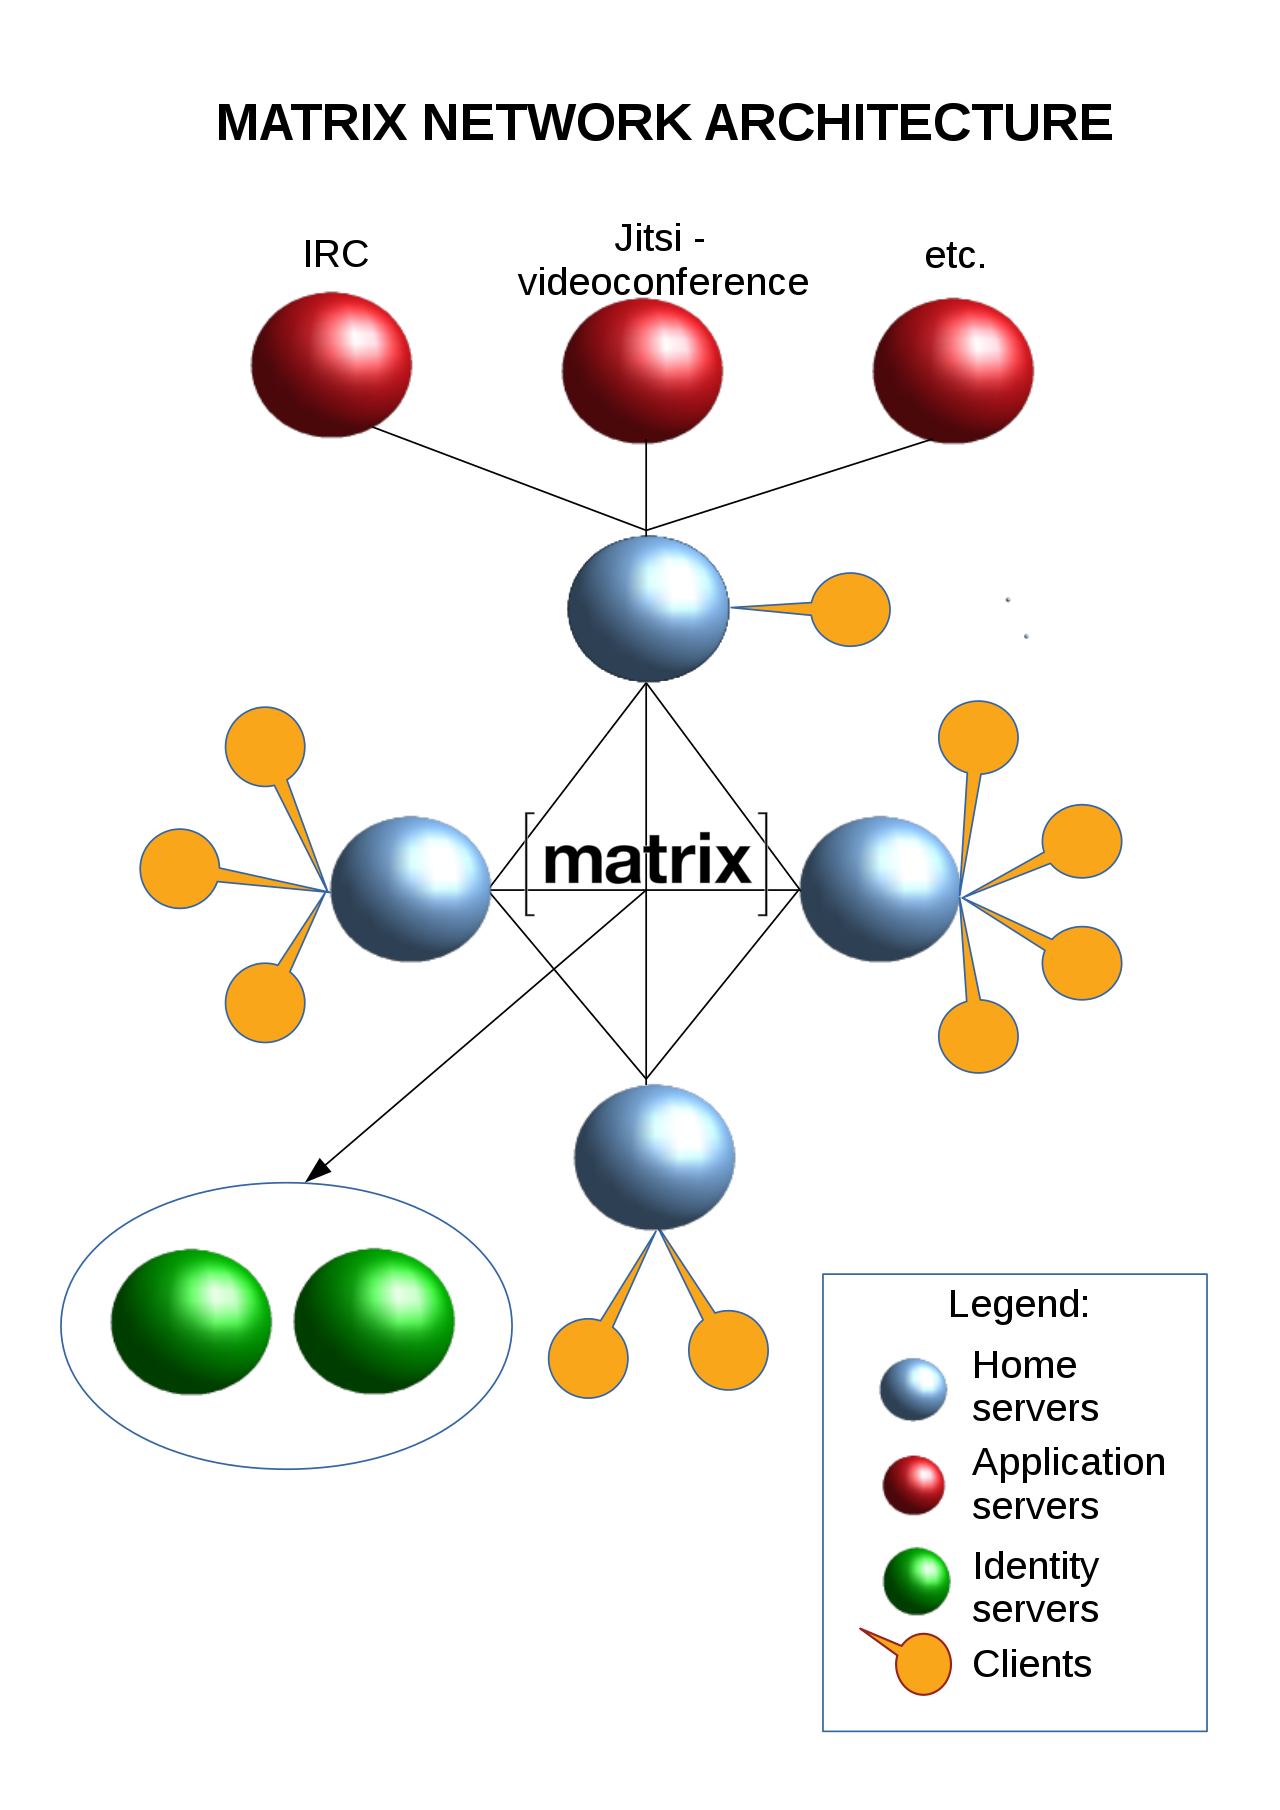
\includegraphics[height=13cm]{graphics/1280px-Diagramme_Matrix_en.png}
    % Titel und Label der Grafik
    \caption[Matrix Netzwerk Architektur]{Matrix Netzwerk Architektur.\footnotemark}
    \label{abb:DHBWLogo}
\end{figure}
\footnotetext{Matrix Netzwerk Architektur Quelle...}

Im Zentrum jeder Matrix Instanz steht der sogenannte Homeserver. Jeder Homeserver stellt dabei eine eigene Instanz des Messengers dar, welcher in Kombination mit einer Datenbank als Speicher und einem Frontend, welches mit den API Schnittstellen des Homeservers kommuniziert, betrieben werden kann. Jeder Nutzer (Client) des Matrixnetzwerks ist dabei einem Homeserver zugeordnet, über welchen sein Account verifiziert wird und welcher für die Sicherung seiner Daten und Chatverläufe zuständig ist. Das besondere hierbei ist, dass die Kommunikation innerhalb von Matrix nicht auf einen einzelnen Homeserver beschränkt ist. Durch ein entsprechendes White bzw Blacklisting kann die Kommunikation mit anderen Homeservern erlaubt beziehungsweise eingeschränkt werden. Matrix geht dabei wie folgt vor:
Der Matrix-Standard spezifiziert RESTful-HTTP-APIs für die sichere Übertragung und Replikation von JSON-Daten zwischen Matrix-fähigen Clients, Servern und Diensten. Diese Daten werden mit einer Signatur im Git-Stil signiert, um Manipulationen zu vermeiden. Das Datenpaket wird mit HTTPS verschlüsselt und mit dem privaten Schlüssel des Servers signiert, um Spoofing zu vermeiden.
Der Client sendet dieses Datenpaket an den gewählten "Raum" auf dem Matrix Homeserver. Dieser repliziert die Daten dann über alle Matrix-Server, die an diesem "Raum" teilnehmen. Somit ist es möglich gezielt zwischen zwei oder mehr Homeservern zu kommunizieren und nur den Inhalt der Chats dieser Räume zwischen den Homeservern auszutauschen, ohne dass sämtliche auf den Datenbanken der Homeserver hinterlegten Chats ausgetauscht werden müssen. Zudem führt dies auch dazu, dass, sollte ein Homeserver aus Gründen nicht erreichbar sein, zum Beispiel durch einen Absturz oder Wartungen an dem System, ist die Kommunikation innerhalb und zwischen den anderen Homeservern des Netzwerks immer noch möglich ist.

Für die Verwaltung von Nutzern ist es möglich einen sogenannten Identity Server mit dem eigenen Homeserver zu verknüpfen, welcher es erlaubt externe Nutzerverwaltungen zur Authentifikation gegenüber dem Homeserver zu Nutzen. Die Basis der Matrix internen Nutzerverwaltung bildet die sogenannte Matrix User IDs (MXID), welche wie folgt aufgebaut ist "@username:homeserver.tld". Diese ist einzigartig für jeden Nutzer. Darauf aufbauend können Third-party IDs (3PIDs) mit der MXID verbunden werden, wie zum Beispiel eine E-Mail-Adresse, eine Handynummer oder ein Display Name, welche die Identifikation einzelner Nutzer vereinfacht. Wird kein Identiy Server mit dem Homeserver verbunden, kann ein Nutzerkonto direkt über den Homeserver erstellt werden. Hierfür kann ein, in der Konfiguration des Homeservers festgelegter 3PID in Kombination mit einem Passwort angegeben werden, worauf der Homeserver den Nutzer anlegt und eine passende MXID erstellt. In der Regel ist es aber wünschenswert eine bereits bestehende Nutzerverwaltung mit dem Homeserver zu verknüpfen, da auf diese Weise die Nutzer keine zusätzlichen Accounts erstellen müssen, weil sie sich über die Nutzerverwaltung authentifizieren können und der Betreiber des Homeservers keine weitere Nutzerverwaltung extra für den Homeserver betreiben muss. Zum Verbinden eines Homeservers mit einer Nutzerverwaltung nutzt Matrix eine Reihe von Schnittstellen. Ein Beispiel für eine unterstütze Schnittstelle ist OpenID Connect, ein offener Standard für ein dezentralisiertes Authentifikation Protokoll. Andere unterstützte Matrix Schnittstellen sind CAS und SAML .

Neben externen Nutzerverwaltungen können auch andere Module an Matrix angebunden werden. Ein Beispiel für ein solches Modul ist das Videokonferenztool Jitsi. Wie auch Matrix basiert Jitsi auf einem Open Source Projekt und bietet einen robusten Dienst für Video und Audio Telefonate, vergleichbar mit anderen Anbietern auf dem Markt, wie zum Beispiel Zoom oder Skype. Matrix bietet zwar auch von Haus die Möglichkeit Video und Audio Telefonate zu führen, dabei ist der Funktionsumfang aber deutlich kleiner als der von Jitsi. Sollte also ein großer Fokus bei der Verwendung der Plattform auf Audio und Videotelefonaten liegen, würde es sinnvoll sein Jitsi als Modul an Matrix anzubinden. Bei Jitsi handelt es sich um nur ein Beispiel der Möglichkeiten Matrix für den eigenen Gebrauch anzupassen. 

\subsubsection{Matrix Verschlüsselung}\label{chapter:aemn}
Die End-to-End-Verschlüsselung in Matrix basiert auf den kryptografischen Modell von Olm und Megolm.
Dadurch können gespeicherte Konversationsdaten nur von Raum-Teilnehmern gelesen werden. Ist dies konfiguriert, sind über Matrix transportierte Daten für Matrix-Server nur als Geheimtext sichtbar. Sie können nur von autorisierten Teilnehmern des Raumes gelesen werden. Die Bibliotheken Olm und Megolm (eine Olm-Erweiterung für größere Chaträume) wurden in einer kryptografischen Review des Unternehmens NCC Group geprüft und die Resultate veröffentlicht. Die Überprüfung wurde finanziert vom Open Technology Fund.

Für den Nutzer bedeutet Matrix Verschlüsselung, dass bei der Erstellung eines neuen Accounts neben einem Passwort zusätzlich eine Passphrase anlegt werden muss, um die von Matrix gespeicherten Nachrichten zu entschlüsseln und somit auf Chatverläufe zugriff zu erhalten.
Die Eingabe der Passphrase ist für jedes neue Device notwendig (alternativ kann das neue Device auch über ein anderes Device, welches bereits entschlüsselt wurde authentifiziert werden).

Die End to End Verschlüsselung bringt eine Reihe von Vorteilen mit sich: Auch bei einem Diebstahl von Nutzername und Passwort sind alte Chatverläufe nicht einsehbar und somit geschützt, die Chats sind ebenfalls in der Datenbank verschlüsselt gespeichert und können somit auch durch einen dirkten Zugriff auf die Datenbank nicht eingesehen werden und die Nachrichten werden ausschließlich in verschlüsselter From versendet und können somit, auch wenn sie abgefangen würden, nicht gelesen werden.

\section{Konzeption des Messengers auf Basis des Matrix Frameworks}\label{chapter:km}
Das folgende Kapitel zeigt wie mithilfe des Matrix Frameworks ein, den aufgestellten funktionalen und gesetzlichen Anforderungen gerechter Messenger, konzipiert werden kann.
Die Implementierung des Matrix Frameworks als Basis des Messenger Dienstes erlaubt es einen Großteil der festgelegten Anforderungen durch das Aufsetzen einer Matrix Instanz und einer entsprechenden Konfiguration des Frameworks zu erfüllen. Da es sich bei Matrix um ein Opensource Projekt handelt, können Anforderungen, welche sich nicht durch eine reine Konfiguration erfüllen lassen, durch Erweiterungen im Code umgesetzt werden.

Dieser Vorgang soll im Folgenden beschrieben werden, um somit ein ausgearbeitetes Konzept zur Umsetzung eines der Zielsetzung dieser Arbeit entsprechenden Messenger Dienst zu erhalten.

\subsection{Konzept zur Umsetzung der funktionalen Anforderungen}\label{chapter:am}
Wie bereits beschrieben, ist einer der herausragenden Vorteile von Matrix, dass neben dem eigentlichen Framework auch ein vollständiges Front- und Backend zur Verfügung gestellt wird. Wie in der Vorstellung von Matrix beschrieben, werden alle funktionalen Anforderungen bereits durch Matrix abgedeckt.

Für das Konzept zur Umsetzung der funktionalen Anforderungen wird deshalb nur eine der Standard-Installation entsprechend, nicht darüber hinaus konfigurierte Matrix Instanz vorausgesetzt, für welche das Webinterface über den Browser im Internet erreichbar ist.
Der Installationsprozess wird in diesem Kapitel nicht weiter beschrieben, da es sich hierbei je nach Betriebssystem und Rechenzentrum um einen für jedes Krankenhaus individuellen Prozess handelt, welcher zudem durch die opensource Community kontinuierlich erweitert und verbessert wird.

Wie das Experteninterview ergab, gibt es eine Vielzahl an möglichen Funktionen, mit welchen der Messenger erweitert werden könnte, um ihn für den Einsatz im Krankenhaus zu optimieren. Auch wenn die Umsetzung dieser nicht unter die Zielsetzung dieser Arbeit fällt, sollte an dieser Stelle angemerkt werden, dass eine Erweiterung des Messengers, dank der Matrix open source Lizenz, gut möglich ist und durch eine aktive Entwickler-Community und steigende Popularität eine kontinuierliche Weiterentwicklung seitens des Opensource Projektes durchaus absehbar ist.

Nach der Installation werden bereits die grundlegenden Funktionen des Messengers in Form eines über den Browser erreichbaren Interfaces zur Verfügung gestellt und können getestet werden. Somit kann sich dank des robusten Matrix Frameworks im folgenden vollständig auf die Umsetzung der gesetzlichen Anforderungen konzentriert werden.

\subsection{Konzept zur Umsetzung der gesetzlichen Anforderungen}\label{chapter:vdmf}
Das folgende Kapitel beschreibt das Konzept zur Umsetzung der gesetzlichen Anforderungen an den Messenger Dienst.
Die Basis hierfür bildet der im Kapitel x erstellte gesetzliche Anforderungskatalog speziell für den Messenger Dienst. Für die Erstellung des Konzeptes wurden alle 37 Anforderungen analysiert und erörtert, wie diese technisch im Messenger durch das Matrix Framework umgesetzt werden können. Die Ansätze wie die Anforderungen technisch umgesetzt werden können wurden im Anforderungskatalog ergänzt. Die erweiterte Tabelle findet sich im Anhang Seite x. 

Die Umsetzungen der einzelnen Anforderungen geschieht dabei durch eine entsprechende Konfiguration einer Reihe von technischen Kernfunktionen seitens Matrix. Neben der Erläuterung wie die jeweilige Anforderung mit Matrix umgesetzt werden kann wird in der Tabelle auf die betroffene Kernfunktion verwiesen. Die Kernfunktionen werden im Folgenden aufgeführt und erläutert.

\subsubsection{Matrix Homeserver YAML}\label{chapter:vdmf}
Die homeserver.yaml Datei innerhalb des Matrix Homeservers ist der zentrale Anlaufpunkt für die Konfiguration des Homeservers.
Über die homeserver.yaml, werden vom anbinden weiterer Komponenten an den Homeserver bis hin zur Einstellung von Upload limits für Media Dateien alle wichtigen Funktionen des Homeservers konfiguriert. Aus diesem Grund wird innerhalb der Beschreibungen zur Umsetzung des Anforderungskatalogs immer wieder auf Einstellungen in der homeserver.yaml verwiesen. Eine Beispielkonfiguration mit Erläuterungen befindet sich im Anhang dieser Arbeit.

\subsubsection{Matrix Policys}\label{chapter:vdmf}
Matrix erlaubt es sogenannte custom Policys anzulegen, über welche sich eine Reihe von Anforderungen an den Messenger Dienst umsetzen lassen, welche sich auf AGBs und Datenschutzhinweise beziehen.
Der Matrix Homeserver kann so konfiguriert werden, dass Benutzern individuelle Richtlinienformulare mit der Schaltfläche "Akzeptieren" präsentiert werden können. Durch Klicken auf "Akzeptieren" wird die Akzeptanz des Benutzers in der Datenbank aufgezeichnet.

Um diese Funktion für Matrix zu aktivieren, muss zunächst die gewünschte Richtlinie im Dateisystem des Homeservers hinterlegt werden.

Die Richtlinie muss dabei die Jinja2 templating language verwenden.

Nachdem die gewünschte Richtlinie auf dem System hinterlegt wurde müssen die folgenden Änderungen an der homeserver.yaml vorgenommen werden:

Nach dem hinterlegen der Policys müssen folgendende Änderungen an der homeserver.yaml vorgenommen werden:

Der folgende Abschnitt muss der homeserver.yaml hinzugefügt werden, damit der Homeserver weiß, wo die gewünschte Policy abgelegt ist und um welche Version der Policy es sich handelt.

\begin{lstlisting}
user_consent:
    template_dir: <Dateipfad zur Policy>
    version: <Versionsnummer>
\end{lstlisting}

Das Tracking ob Nutzer der Policy zugestimmt haben kann mit der folgenden Konfiguration ermöglicht werden.

\begin{lstlisting}
user_consent:
    require_at_registration: true
    policy_name: <Name der Policy>
\end{lstlisting}

Matrix zudem so konfiguriert werden, dass er Dienste erst dann wieder genutzt werden kann, wenn der Policy zugestimmt wurde.
Dies geschieht über eine weitere Anpassung an der homeserver.yaml.

\begin{lstlisting}
user_consent:
    block_events_error: >-
        <Individuelle Nachricht die dem Nutzer angezeigt werden soll>
\end{lstlisting}

Diese Beschreibung soll dazu dienen ein grundsätzliches Verständis dafür zu bekommen, wie Policys in Matrix umgesetzt werden können. Die vollständige Entwicklerdokumentation für Policys befindet sich im Anhang.

\subsubsection{Matrix Message retention policies}\label{chapter:vdmf}
Innerhalb der Matrix homeserver.yaml des Matrix Homeservers kann eine sogenannte retention Policy festgelegt werden, welche die maximale Speicherdauer für alle über den Server versendeten Nachrichten festlegt. Beispielsweise kann eine retention Policy von 30 Tagen dafür sorgen, dass Nutzer nur die Nachrichten der letzten 30 Tage über den Messenger einsehen können und auch nur die Nachrichten der letzten 30 Tage in der Matrix Datenbank gespeichert werden. Die Konfiguration dieser Policy funktioniert wie folgt:

Neben einer serverweiten retention Policy kann auch eine retention Policy für individuelle Räume festgelegt werden, welche nach dem gleichen Prinzip funktioniert und von den Administratoren des entsprechenden Raumes aktiviert werden kann. Diese Funktion kann von Nutzen sein, wenn Räume zum Versenden besonders sensibler Daten vorgesehen sind. Hier könnte die retention auf zum Beispiel 48 Stunden gesetzt werden, um sicher zu gehen, dass die Daten nicht länger als unbedingt notwendig im Messenger gespeichert bleiben. Die retention Policy für individuelle Räume kann von Administratoren bei den Raum Einstellungen im Developer Feld mit dem folgenden Befehl festlegen:

In der homeserver.yaml kann muss die retention Funktion aktiviert werden.

\begin{lstlisting}
retention:
    enabled: true
\end{lstlisting}

Nachdem aktivieren kann eine serverweite retention Policy wie im folgenden Beispiel über die homeserver.yaml konfiguriert werden.

\begin{lstlisting}
default_policy:
    max_lifetime: 30d
\end{lstlisting}

Nach einer Konfiguration wie in diesem Beispiel werden alle Nachrichten die älter als 30 Tage sind von der Datenbank des Homeservers gelöscht.

\subsubsection{Matrix Nutzerverzeichnis Anbindung am Beispiel von IBM APP ID}\label{chapter:vdmf}
Wie bereits in Kapitel x beschrieben kann Matrix durch eine Reihe von Standards mit externen Nutzerverwaltungen verbunden werden.
Je nach gewähltem Standard und Nutzerverwaltung kann sich der Prozess zur Anbindung unterscheiden. Um den Nutzen und die Funktionsweise einer externen Nutzerverwaltung im Zusammenhang mit Matrix zu erläutert wird der Prozess im Folgenden beispielhaft durch die Anbindung des IBM Service APP ID per OIDC an eine Matrix Instanz demonstriert. Bei APP ID handelt es sich um einen Service, welcher als Connector zwischen Applikation und Nutzerverwaltungen verstanden werden kann. APP ID kann über eine Reihe von Schnittstellen mit Programmen oder Web Applikationen verbunden werden um deren Authentifikationsprozesse zu managen. Einmal angebunden können über APP ID bausteinartig Authentifikationsmethoden der entsprechenden Software hinzugefügt werden. Beispiele hierfür sind Login per Google oder Facebook Account, die APP ID eigene Nutzerverwaltung oder über eine weitere externe Nutzerverwaltung, welche an APP ID angebunden wurde. Dabei bietet APP ID zudem eine Reihe von Sicherheitsfunktionen wie 2 Faktor Authentifikation oder das Monitoring von Nutzeraktivitäten.
Im Folgenden wird gezeigt, wie APP ID an eine Matrix Instanz angebunden werden kann:

\subsubsection{Matrix Nutzer Administration}\label{chapter:vdmf}
Für eine Administration von Chat Räumen bietet Matrix ein umfassendes Set an Rechten (siehe Abbildung) und Herachiebenen mit denen es möglich ist die Kommunikation im jeweiligen Chatraum zu managen. Matrix regelt die Vergabe der Rechte dabei vie folgt: Die Person, welche einen Raum anlegt ist ihr Administrator, von dieser Person ausgehend können dann alle Rechte wie gewünscht verteilt werden. Somit entsteht zwar ein organisatorischer Aufwand, da Gruppen einzeln mit den gewünschten Rechten konfiguriert werden müssen, auf der anderen Seite gibt es aber den Nutzern der Plattform eine wesentlich höheren gestaltungfreiraum innherlab der Gruppen. Dadurch das die Rechtevergabe nicht auf externen Systemen beruht, sondern selbstständig gemanaget werden kann entsteht ein hoher Grad an flexibilität bei der Einrichtung von Gruppen, der für einen Messanger Dienst angemessen ist.

% Einfügen einer Grafik
\begin{figure}[htb]
    % Zentrierung
    \centering
    % Einfügen der Datei, mit angepasster Höhe
    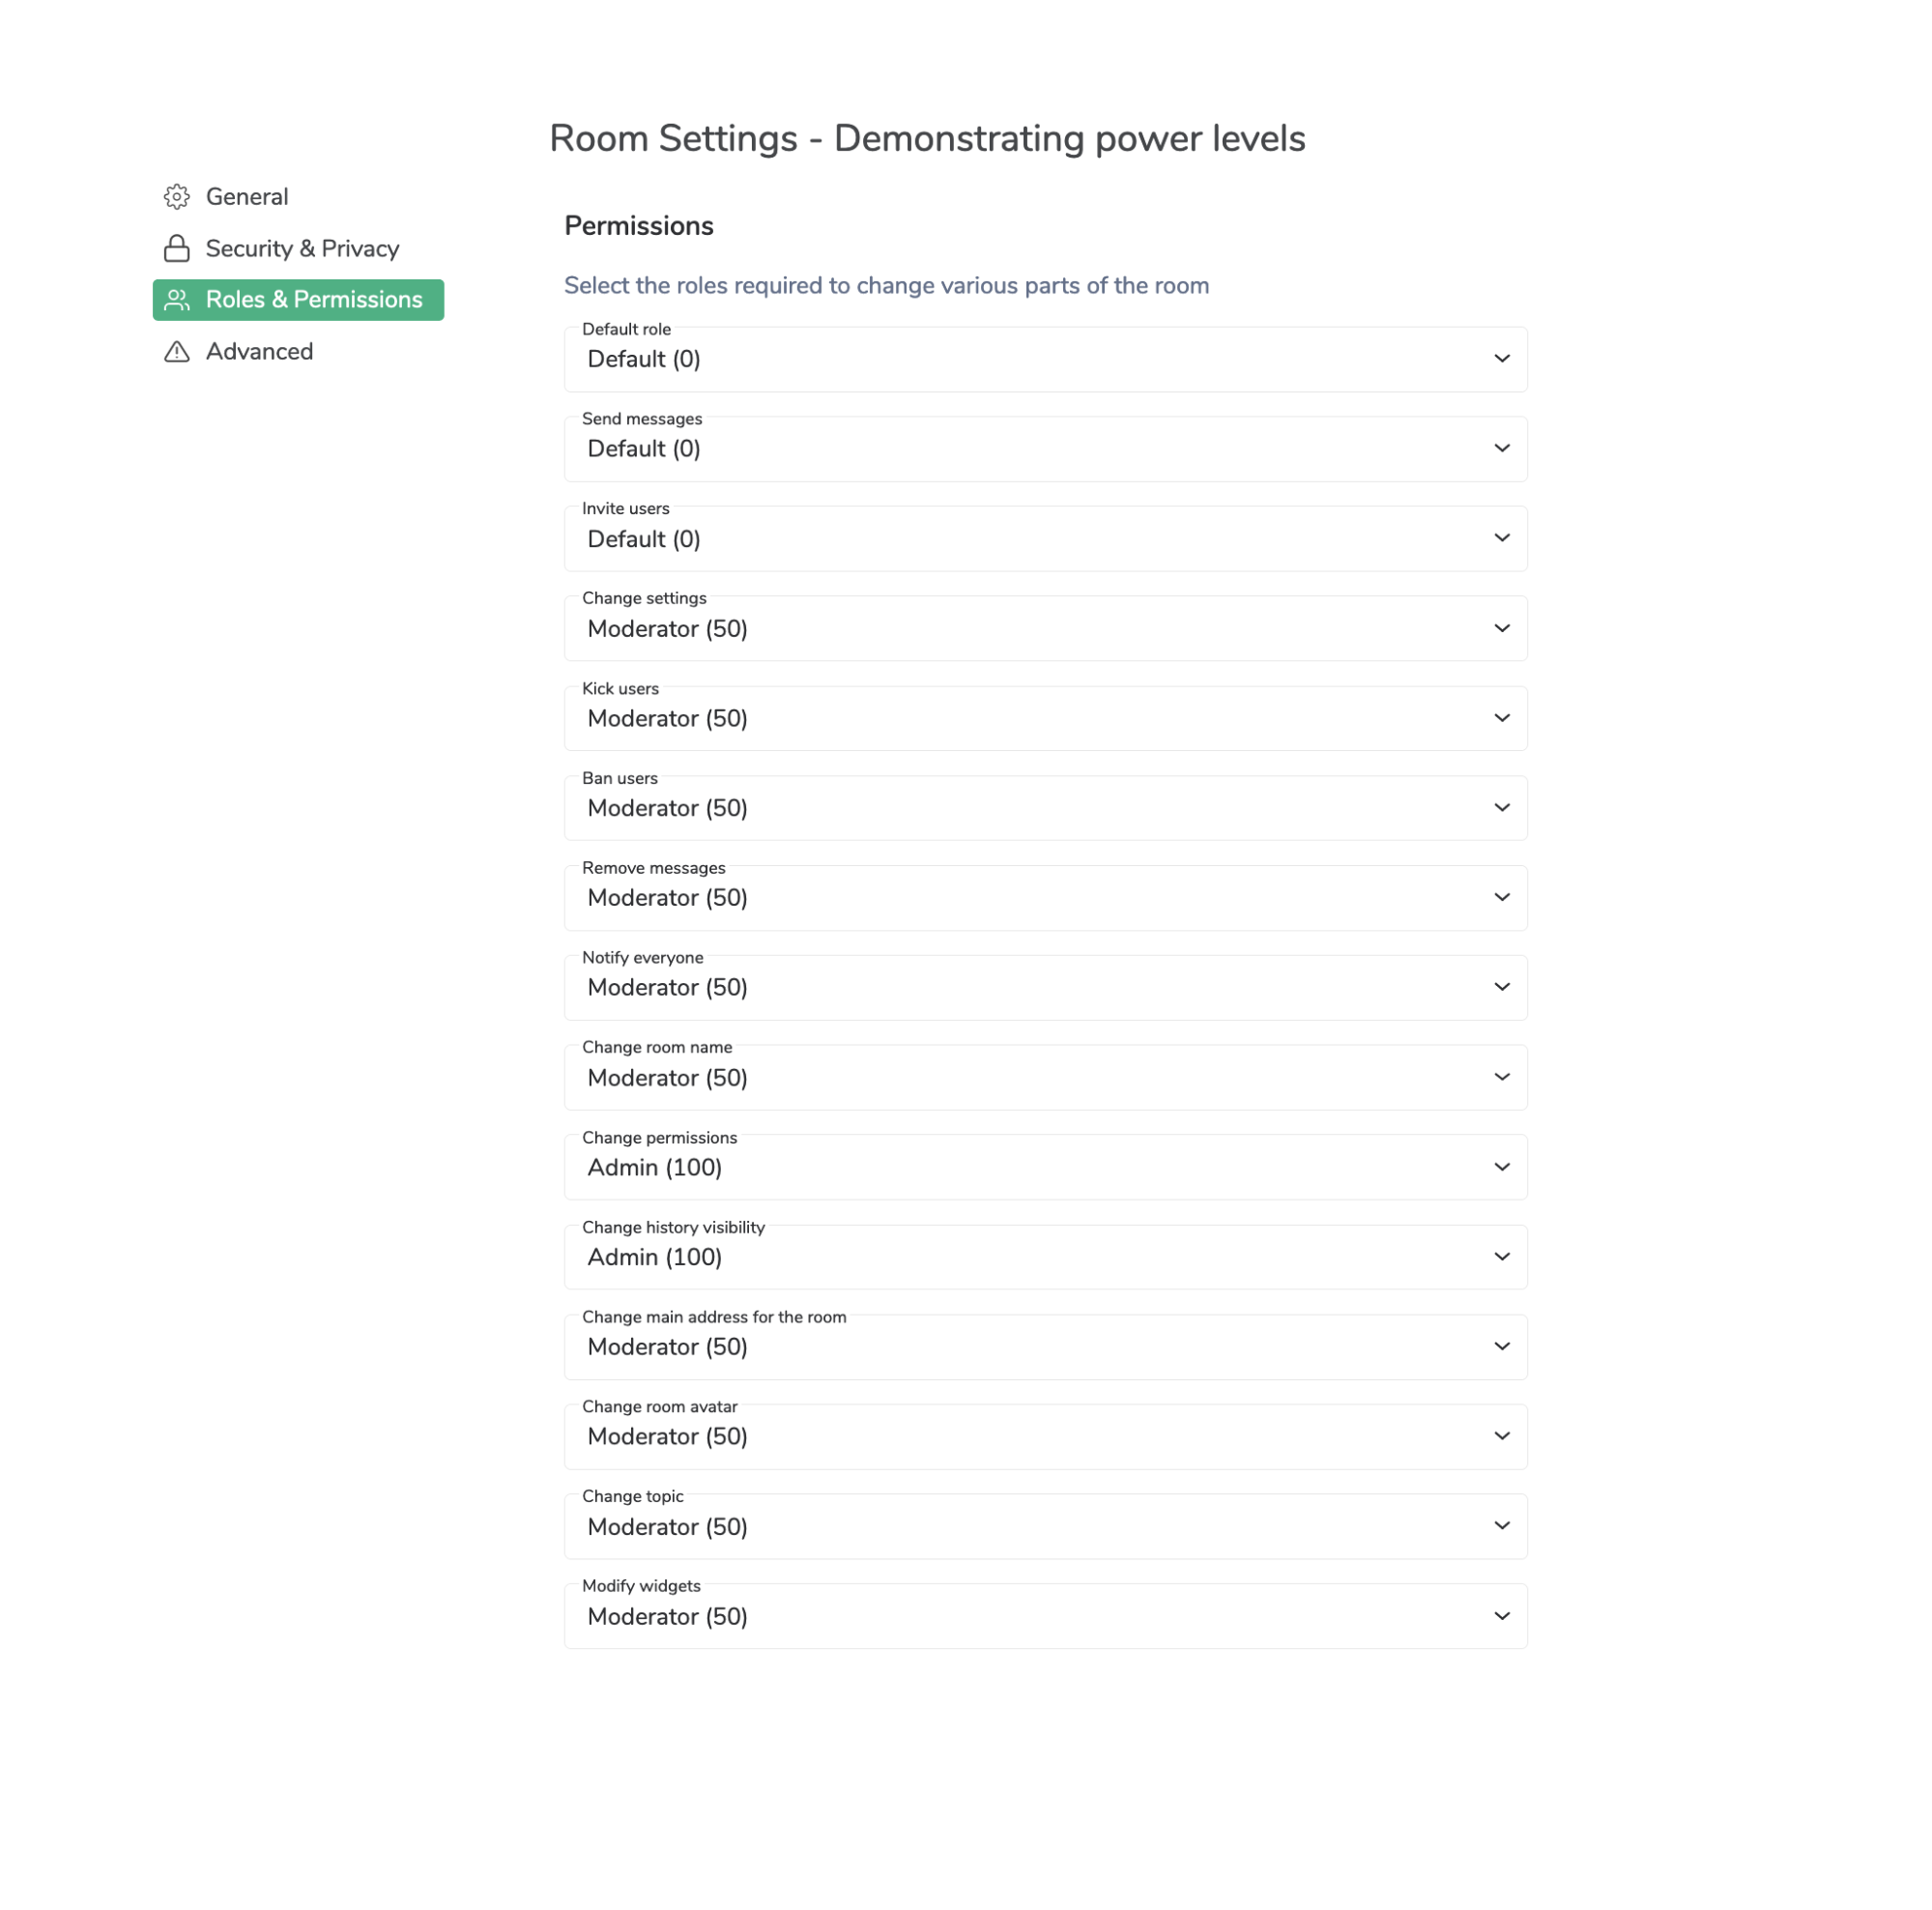
\includegraphics[height=15cm]{graphics/moderation3.png}
    % Titel und Label der Grafik
    \caption[Matrix Administrationsoptionen]{Matrix Administrationsoptionen.\footnotemark}
    \label{abb:UI}
\end{figure}
